\documentclass{beamer}
\usepackage{amsmath,amssymb}
\usepackage{graphicx}
\usepackage{siunitx}
\sisetup{per-mode=symbol}
\usepackage{gvv}
\usepackage{listings}
\usepackage{xcolor}

% Code style
\lstset{
  basicstyle=\ttfamily\scriptsize,
  breaklines=true,
  frame=single,
  numbers=left,
  numberstyle=\tiny,
  keywordstyle=\color{blue},
  commentstyle=\color{green!50!black},
  stringstyle=\color{red!60!black},
  showstringspaces=false
}

\title{Matrix 4.4.11}
\author{ai25btech11015 -- M Sai Rithik}
\date{}

\begin{document}
\maketitle

\begin{frame}
    \frametitle{Question}
    The line segment joining the points \(A(2,1)\) and \(B(5,-8)\) is trisected at the points \(P\) and \(Q\), where \(P\) is nearer to \(A\).  
    If \(P\) lies on the line
    \[
    2x - y + k = 0,
    \]
    find the value of \(k\).  
    (Use matrix/linear algebra concepts only.)
\end{frame}

\begin{frame}
    \frametitle{Step 1: Vectors}
    Write the position vectors:
    \begin{align}
    \Vec{A} &= \myvec{2 \\ 1}, \quad
    \Vec{B} = \myvec{5 \\ -8} \label{eq:AB-beamer}
    \end{align}

    Difference:
    \begin{align}
    \Vec{B} - \Vec{A} = \myvec{3 \\ -9} \label{eq:BA-beamer}
    \end{align}
\end{frame}

\begin{frame}
    \frametitle{Step 2: Trisection point \(P\)}
    First trisection point:
    \begin{align}
    \Vec{P} &= \Vec{A} + \tfrac{1}{3}(\Vec{B}-\Vec{A}) \label{eq:Pdef-beamer}
    \end{align}

    Substitution:
    \begin{align}
    \Vec{P} &= \myvec{2 \\ 1} + \tfrac{1}{3}\myvec{3 \\ -9}
    = \myvec{2 \\ 1} + \myvec{1 \\ -3}
    = \myvec{3 \\ -2} \label{eq:Pcoord-beamer}
    \end{align}
\end{frame}

\begin{frame}
    \frametitle{Step 3: Line condition}
    Coordinates of \(P\) are \((3,-2)\).  
    Substituting into the line:
    \begin{align}
    2(3) - (-2) + k &= 0 \label{eq:plug-beamer}
    \end{align}

    Simplify:
    \begin{align}
    8 + k &= 0 \quad \Longrightarrow \quad k = -8 \label{eq:kval-beamer}
    \end{align}
\end{frame}

\begin{frame}
    \frametitle{Final Answer}
    \[
    \boxed{k = -8}
    \]
\begin{figure}[h!]
    \centering
    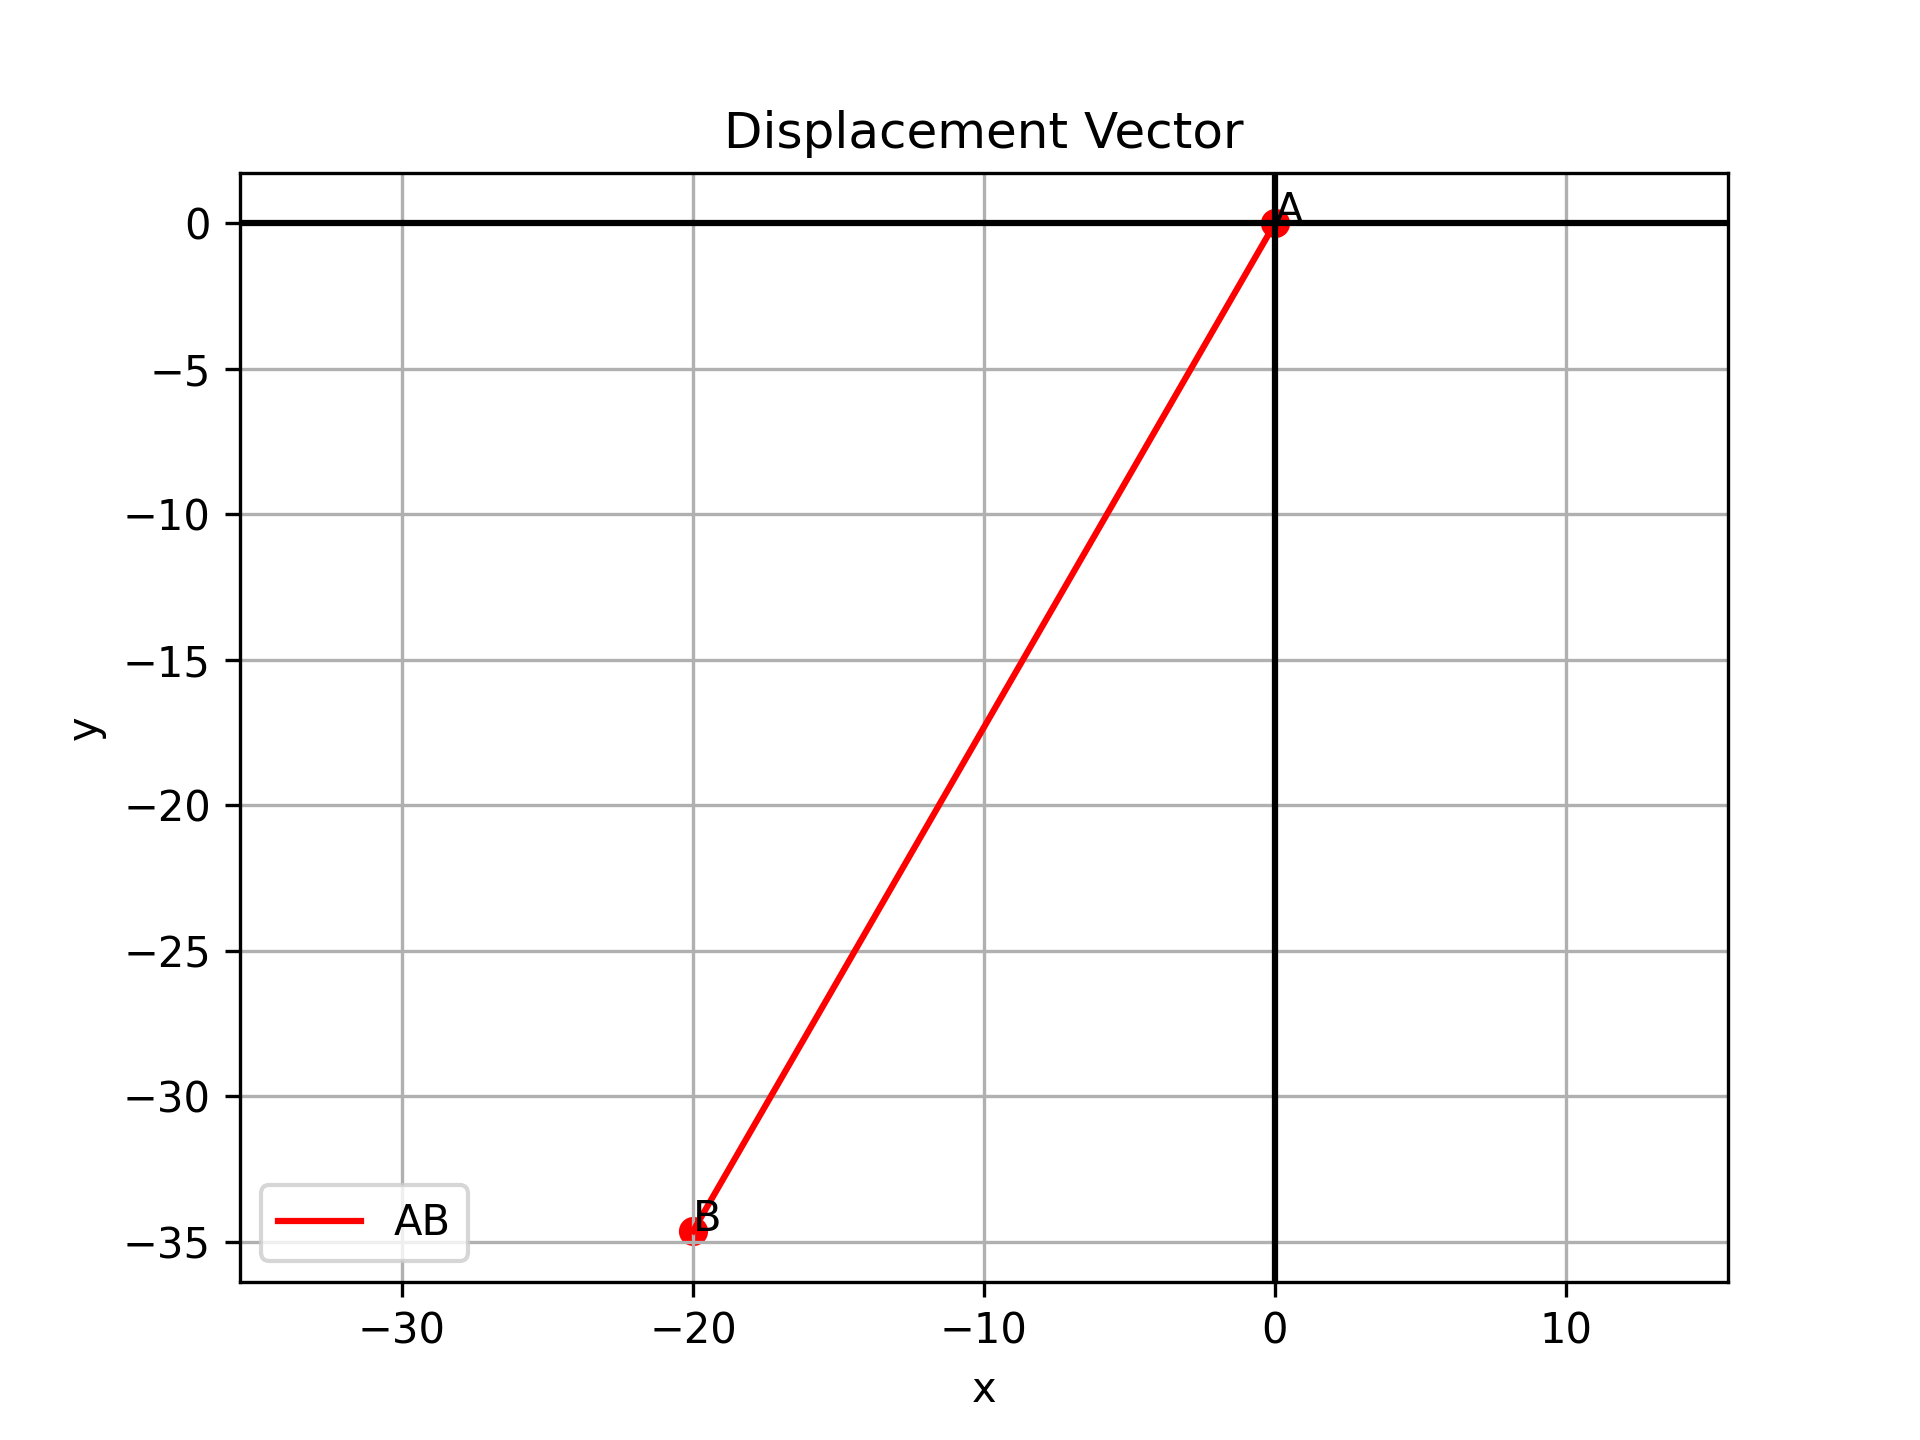
\includegraphics[width=0.65\linewidth]{figs/fig.png}
    \caption{}
\end{figure}

\end{frame}

\end{document}
